\documentclass[a4paper,10pt]{article}
\usepackage[utf8]{inputenc}
\usepackage[margin=0.75in]{geometry}
\usepackage{hyperref}
% \usepackage{url}
\usepackage{color}
\usepackage{listings}
\usepackage{ifpdf}
\usepackage{graphicx}

\usepackage{caption}
\usepackage{subcaption}

\parskip 0pt
\parindent 0pt
% \renewcommand{\indent}{\hspace{2cm}}

\definecolor{gray}{rgb}{.6,.6,.6}
\definecolor{orange}{rgb}{1,0.5,0}
\definecolor{grayish}{rgb}{.775, .775, .775}

\definecolor{dkgreen}{rgb}{0,0.6,0}
\definecolor{mauve}{rgb}{0.58,0,0.82}

\lstdefinelanguage{sh}{basicstyle=\ttfamily\color{white}, backgroundcolor=\color{black}, breaklines=true} 

\ifpdf
\lstdefinelanguage{rr}{language=R, 
                       basicstyle=\ttfamily\color{black}, 
		       backgroundcolor=\color{grayish}, 
		       frame=single, 
		       breaklines=true, 
		       tabsize=2,
                      keywordstyle=\color{blue},
		      commentstyle=\color{dkgreen},
		      stringstyle=\color{mauve}
} 

\else

\lstdefinelanguage{rr}{basicstyle=\ttfamily\color{black}, 
		       backgroundcolor=\color{grayish}, 
		       frame=single, 
		       breaklines=true, 
		       tabsize=2
%                       keywordstyle=\color{blue},
% 		      commentstyle=\color{dkgreen},
% 		      stringstyle=\color{mauve}
} 

\fi


\lstnewenvironment{rr}{%
  \lstset{%
     language = R,%
      style    = default,%
    }%
 }{}





\hypersetup{
    pdfnewwindow=true,      % links in new window
    colorlinks=true,       % false: boxed links; true: colored links
    linkcolor=blue,          % color of internal links
    filecolor=blue,      % color of file links
    urlcolor=blue           % color of external links
}

\title{Quick Start Guide for R on Nautilus}
\author{Drew Schmidt}

% \setcounter{secnumdepth}{0}

% \newcommand{\HRule}{\underline{\ \ \ \ \ \ \ \ \ \ \ \ \ \ \ \ \ \ \ \ }}
% \newcommand{\lsc}[1]{ \ \\ \ \\ \ \\ \ \\ \begin{flushright}\hyperlink{thetop}{Return to top} \end{flushright} \section{#1}}
\newcommand{\lsc}[1]{ \ \\ \section{#1}}
% \newcommand{\lsuc}[1]{ \ \\ \ \\ \begin{flushright}\hyperlink{thetop}{Return to top} \end{flushright} \subsection{#1}}
\newcommand{\lsuc}[1]{\subsection{#1}}

\begin{document}

\ifpdf \else
\Css{div.lstlisting{
    font-family: monospace;
    white-space: nowrap; margin-top:0.5em;
    margin-bottom:0.5em;
    color: black;
    background-color: gray;
  } 
  div.verbatim{
    font-family: monospace;
    white-space: nowrap; margin-top:0.5em;
    margin-bottom:0.5em;
    color: white;
    background-color: black;
  }
}


\Preamble{xhtml}
  \Configure{graphics*}  
         {pdf}  
         {\Needs{"convert \csname Gin@base\endcsname.pdf  
                               \csname Gin@base\endcsname.png"}%  
          \Picture[pict]{\csname Gin@base\endcsname.png}%  
         }  
\fi

\maketitle
\hypertarget{thetop}{\ }
\tableofcontents



%%%%%%%%%%%%%%%%%%%%%%%%%%%%%%%%%%%%%%%%%%%%%%%%%%%%%%%%%%%%%%%%%%%%%%%%%%%%%%%%%%%%%%%%%%%%%%%%%
%%%%%%%%%%%%%%%%%%%%%%%%%%%%%%%%%%%%%%%%%%%%%%%%%%%%%%%%%%%%%%%%%%%%%%%%%%%%%%%%%%%%%%%%%%%%%%%%%
%%%%%%%%%%%%%%%%%%%%%%%%%%%%%%%%%%%%%%%%%%%%%%%%%%%%%%%%%%%%%%%%%%%%%%%%%%%%%%%%%%%%%%%%%%%%%%%%%

\section{Introduction to HPC and Its View from R}
\makesubcontentsslides

\subsection{An R and \protect\pbdR View of Parallel Hardware and Software}
\makesubcontentsslidessec

\begin{frame}{R Interfaces to Low-Level Native Tools}
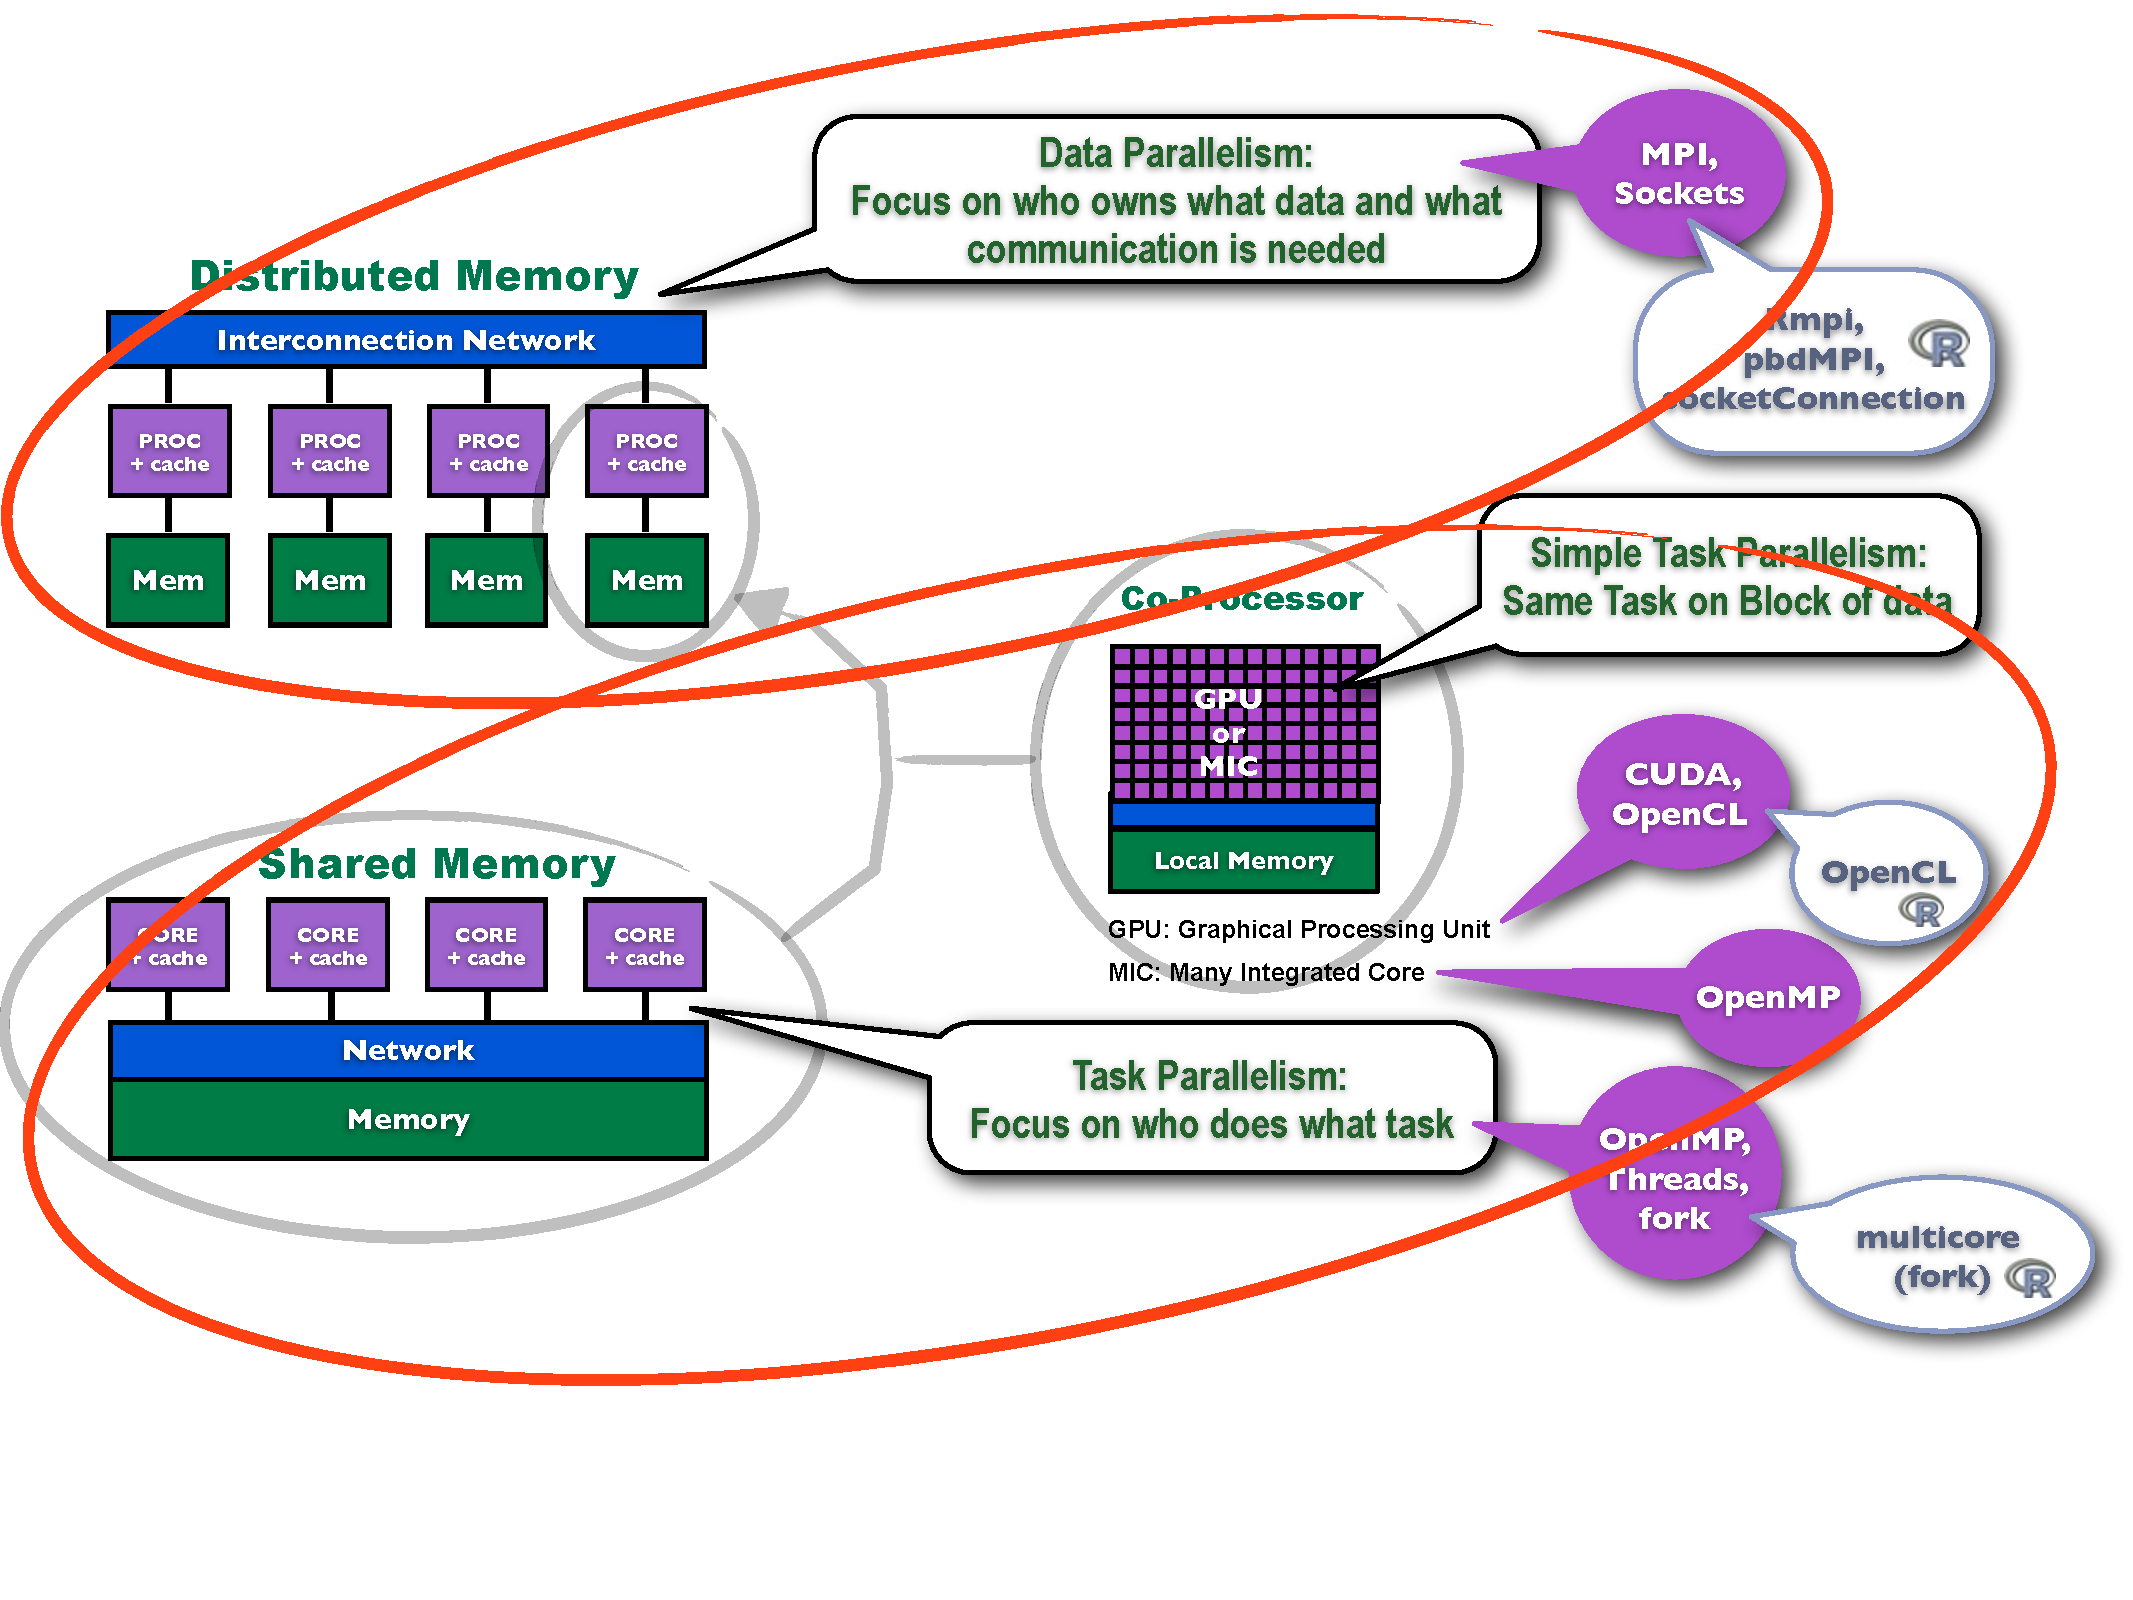
\includegraphics[height=\textheight]
{../common/pics/hardware/ParallelHardware10.pdf}
\end{frame}

\begin{frame}{HPC Libraries: 30+ Years of Research}
\includegraphics[height=\textheight]
{../common/pics/hardware/ParallelHardware25.pdf}
\end{frame}

\begin{frame}{R and \pbdR R Interfaces to HPC Libraries}
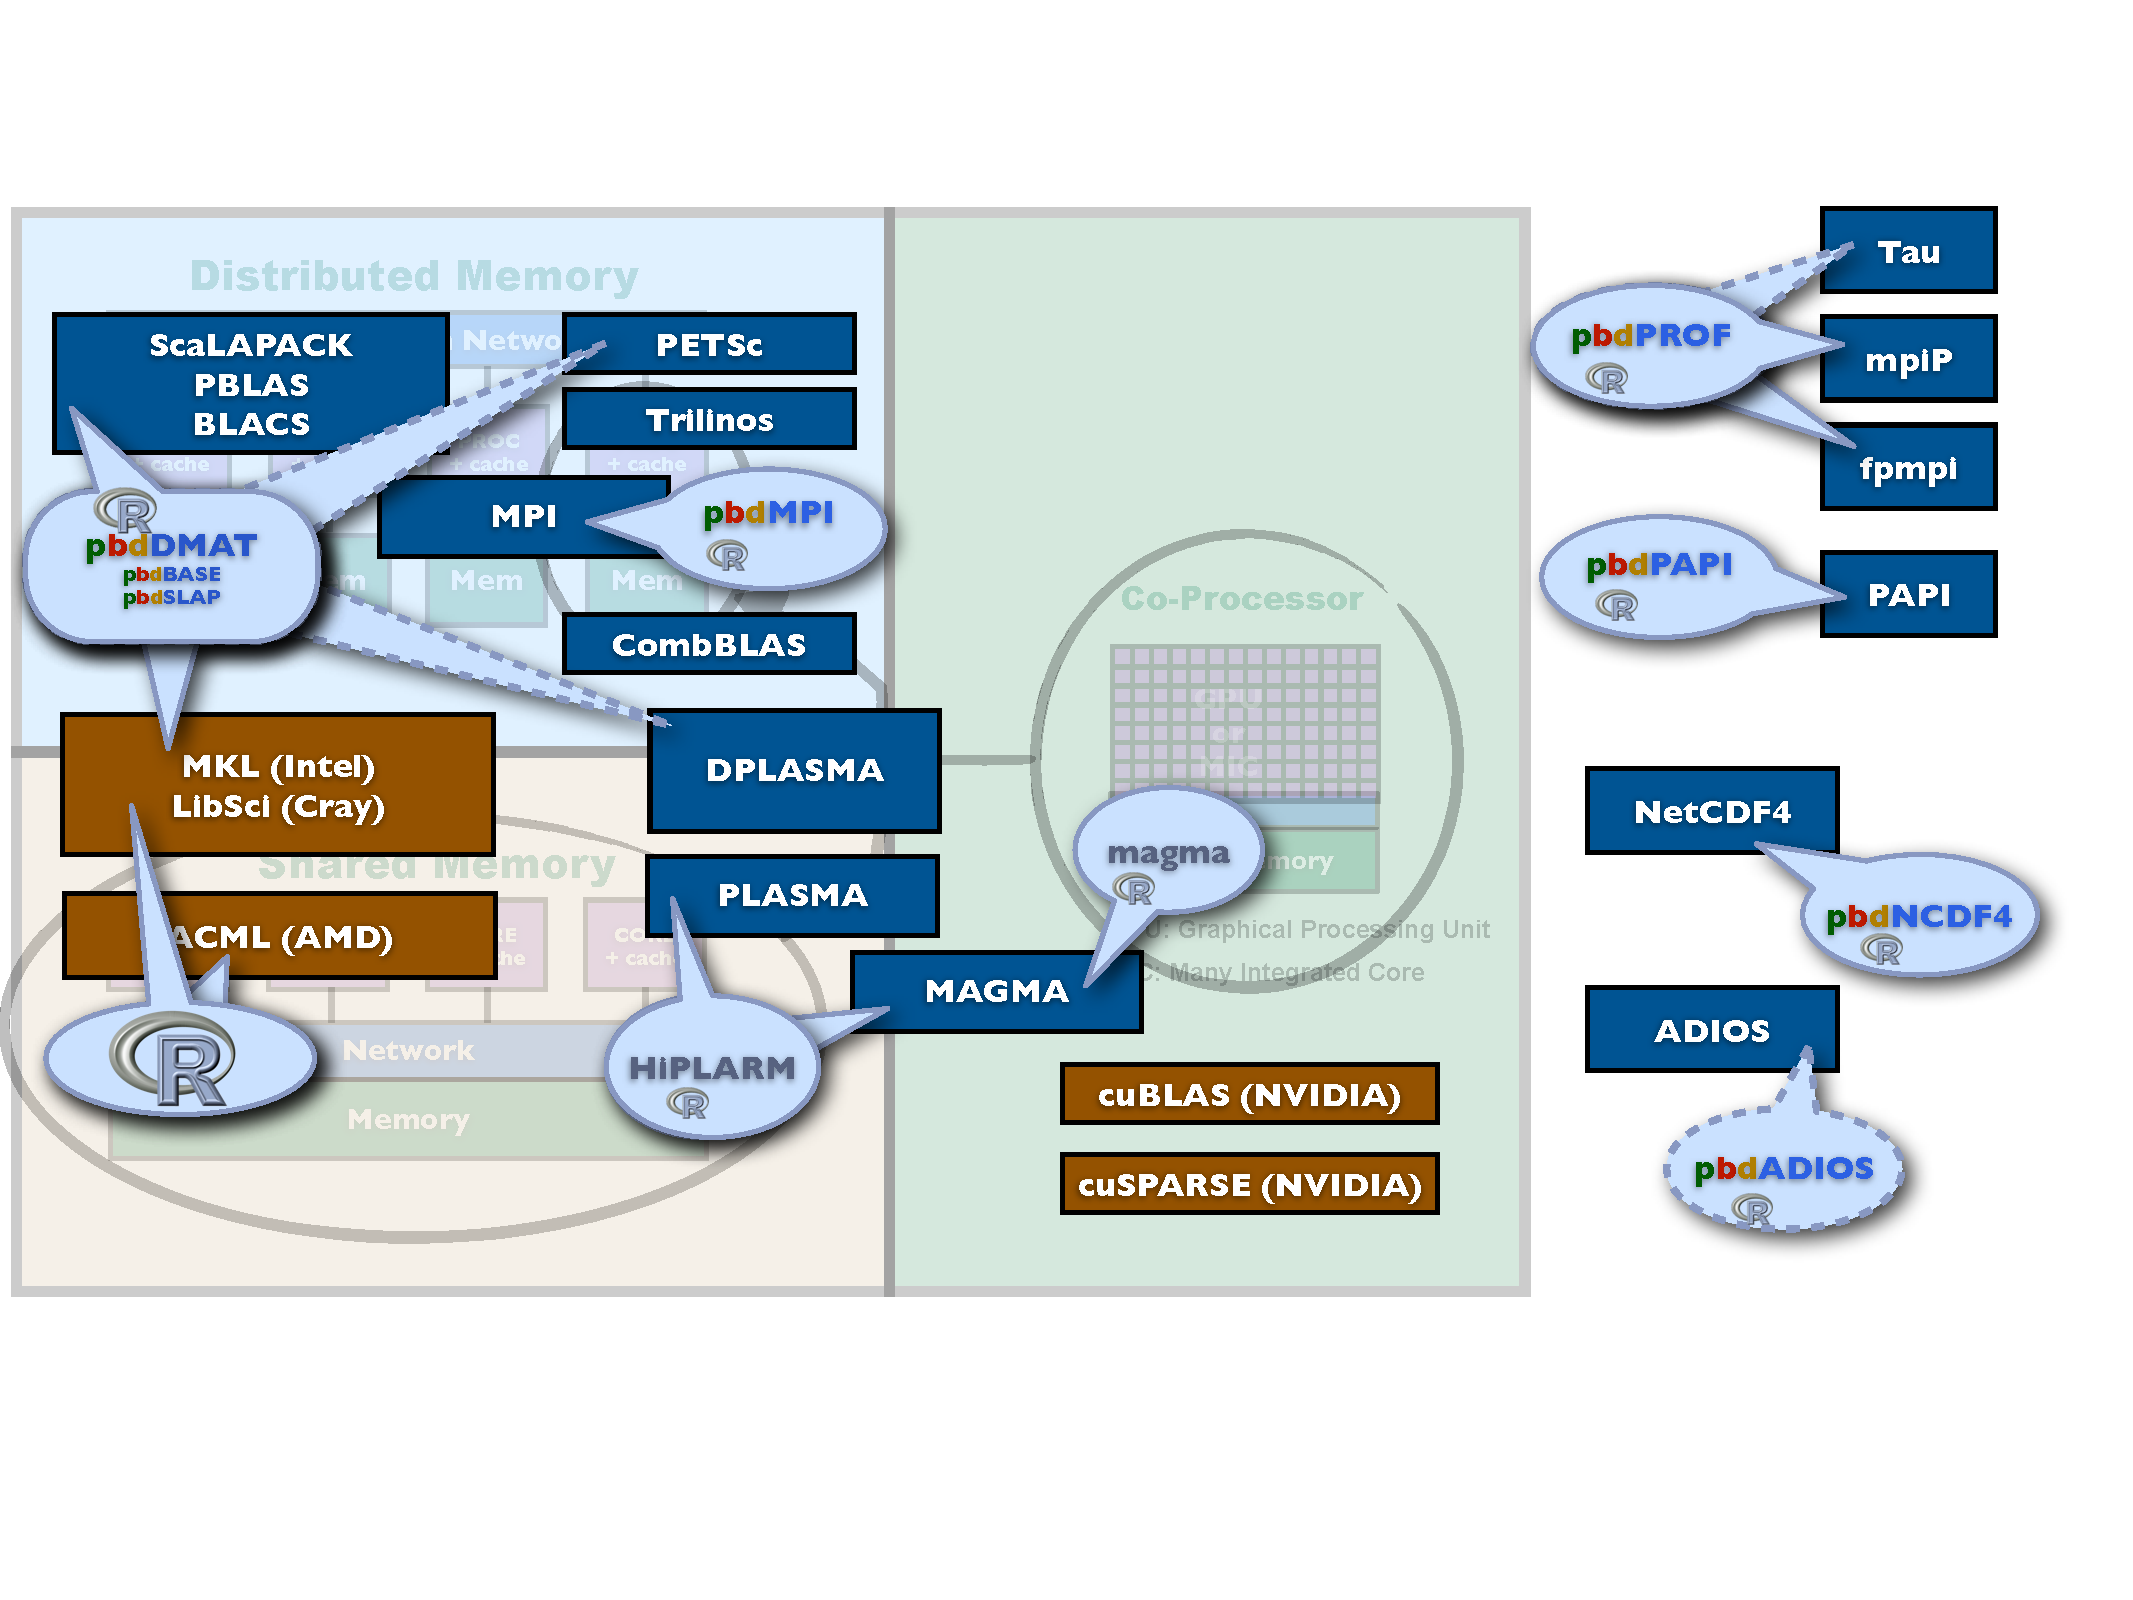
\includegraphics[height=\textheight]
{../common/pics/hardware/ParallelHardware26.pdf}
\end{frame}

\begin{frame}{Big Data and Little Data}
\begin{minipage}{10cm}
  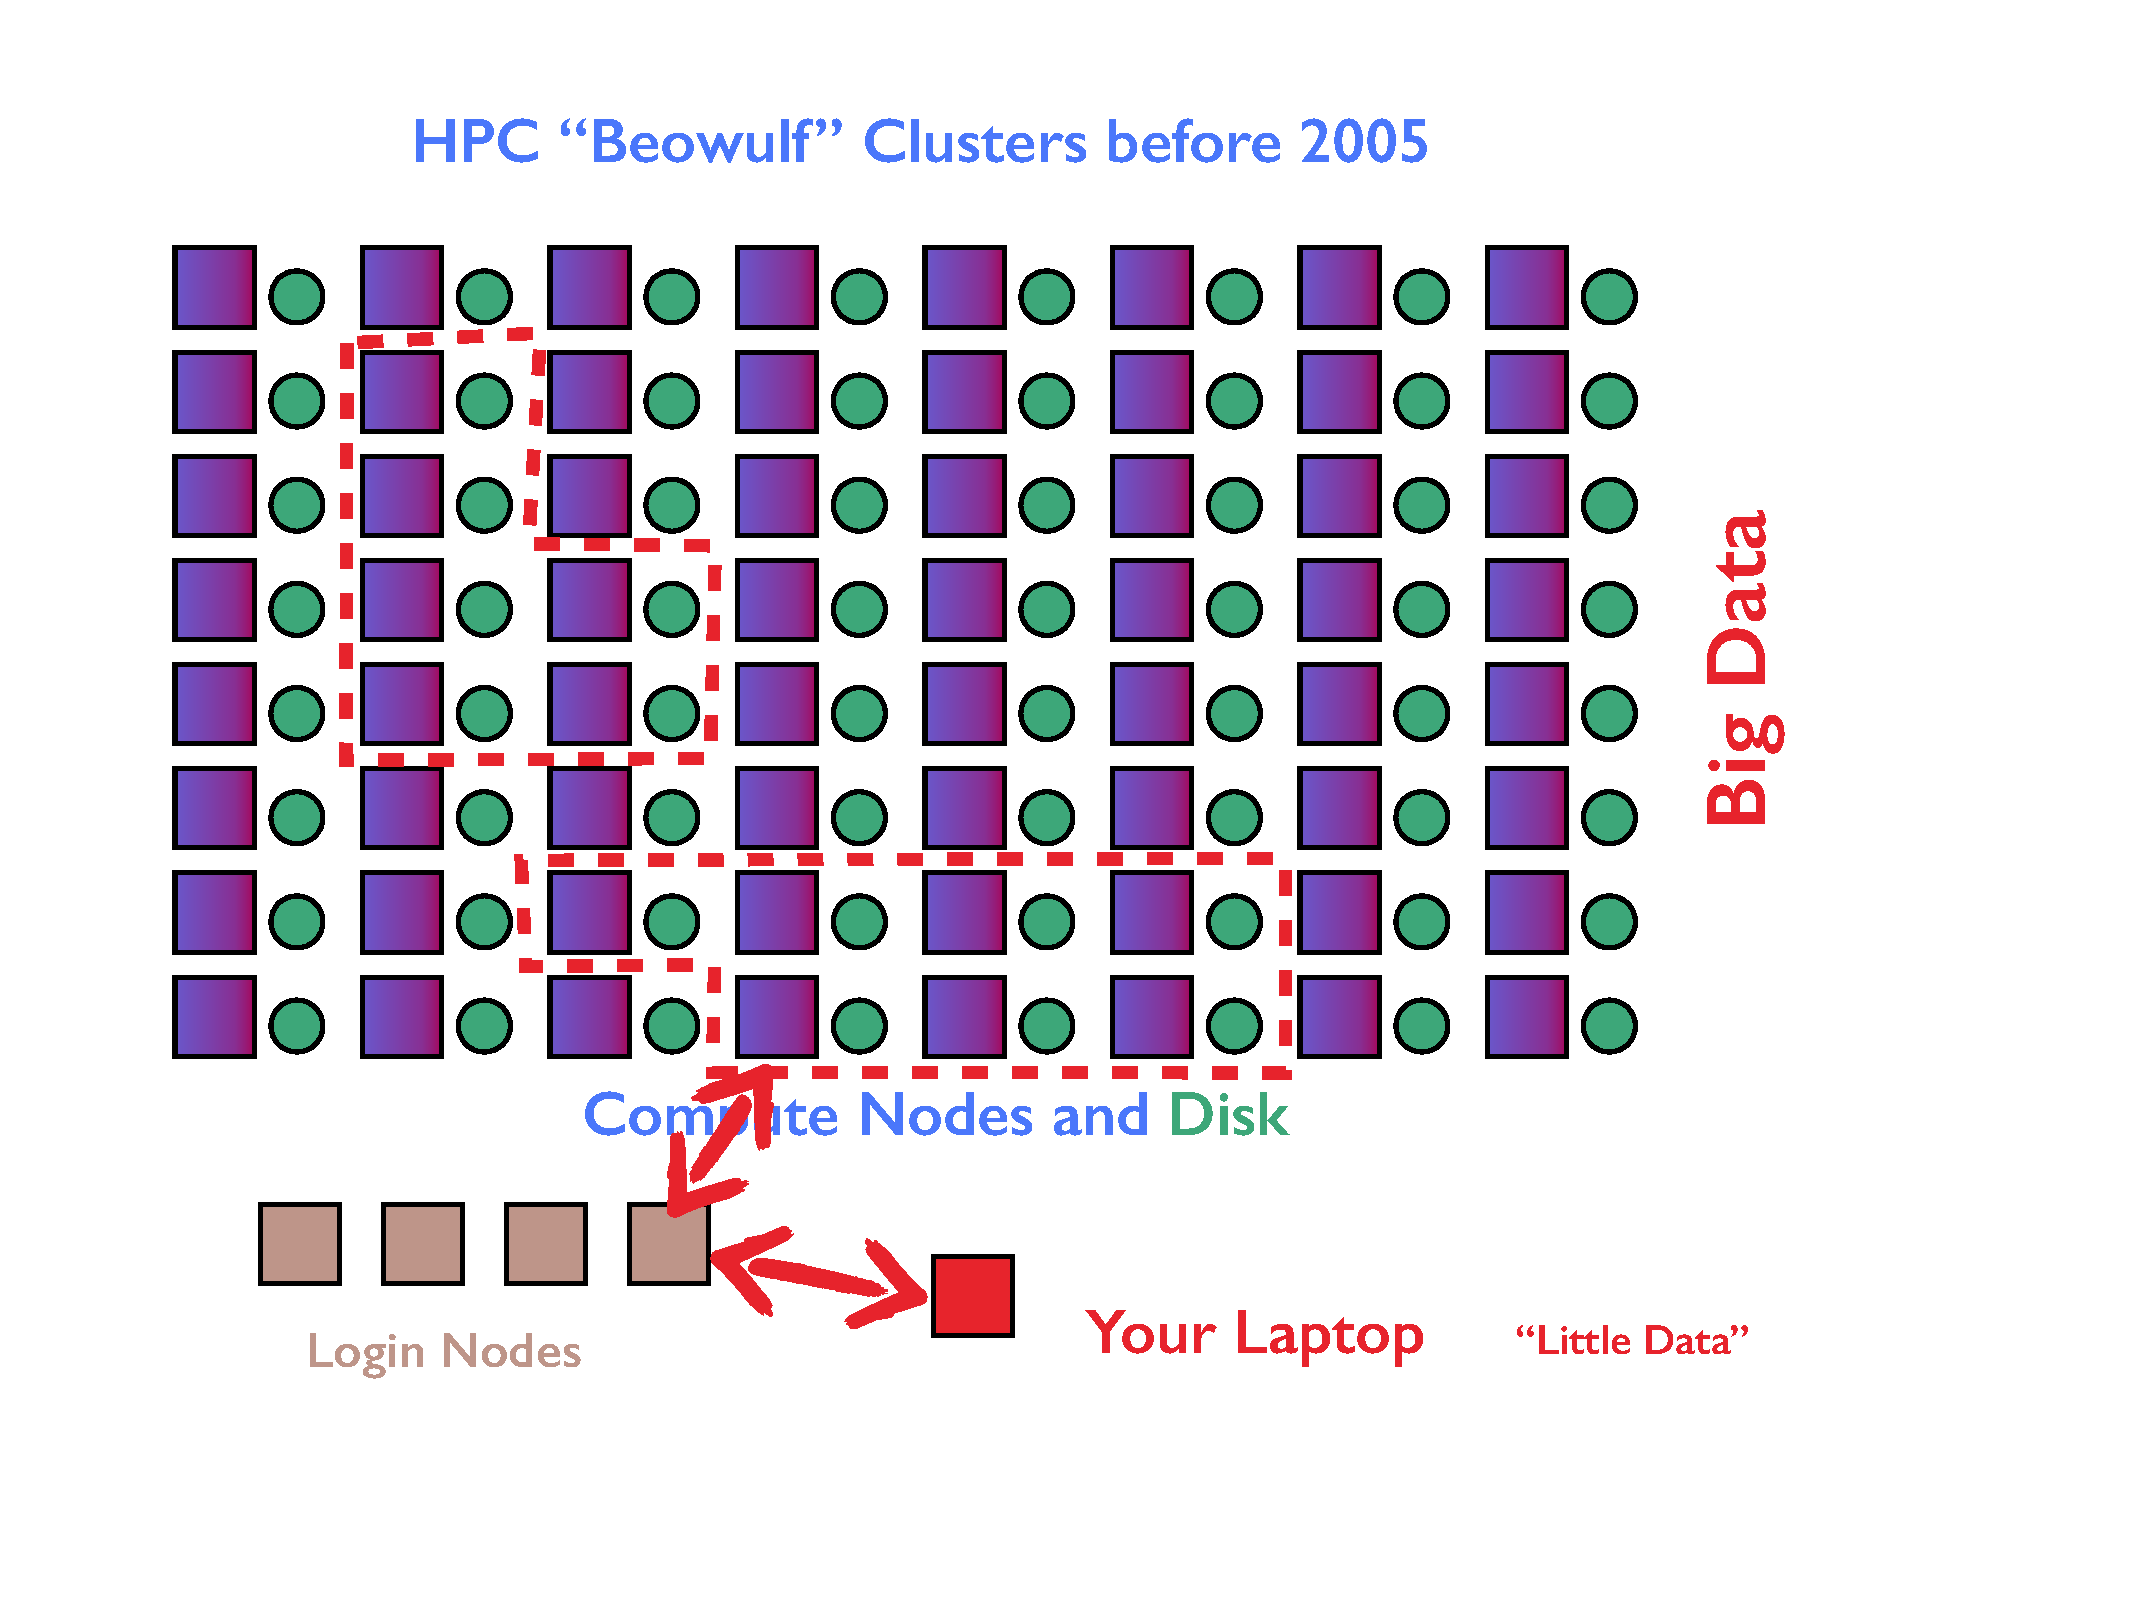
\includegraphics[height=0.9\textheight]
  {../common/pics/hardware/ParallelHardware22.pdf}\hfill
\end{minipage}
\begin{minipage}{5cm}\small
  \begin{block}{Analysis Workflow}\pause
    \begin{itemize}[<+-|alert@+>]
    \item Get Big Data
      \begin{itemize}
      \item Parallel data reader
      \item Parallel data generator
      \end{itemize}
    \item Write analysis script
    \item Graphics to display results
    \item Profile and optimize code
    \end{itemize}
  \end{block}
\end{minipage}
\end{frame}

\begin{frame}{Hadoop: Will it merge with HPC in the future?}
\begin{minipage}{8.5cm}
  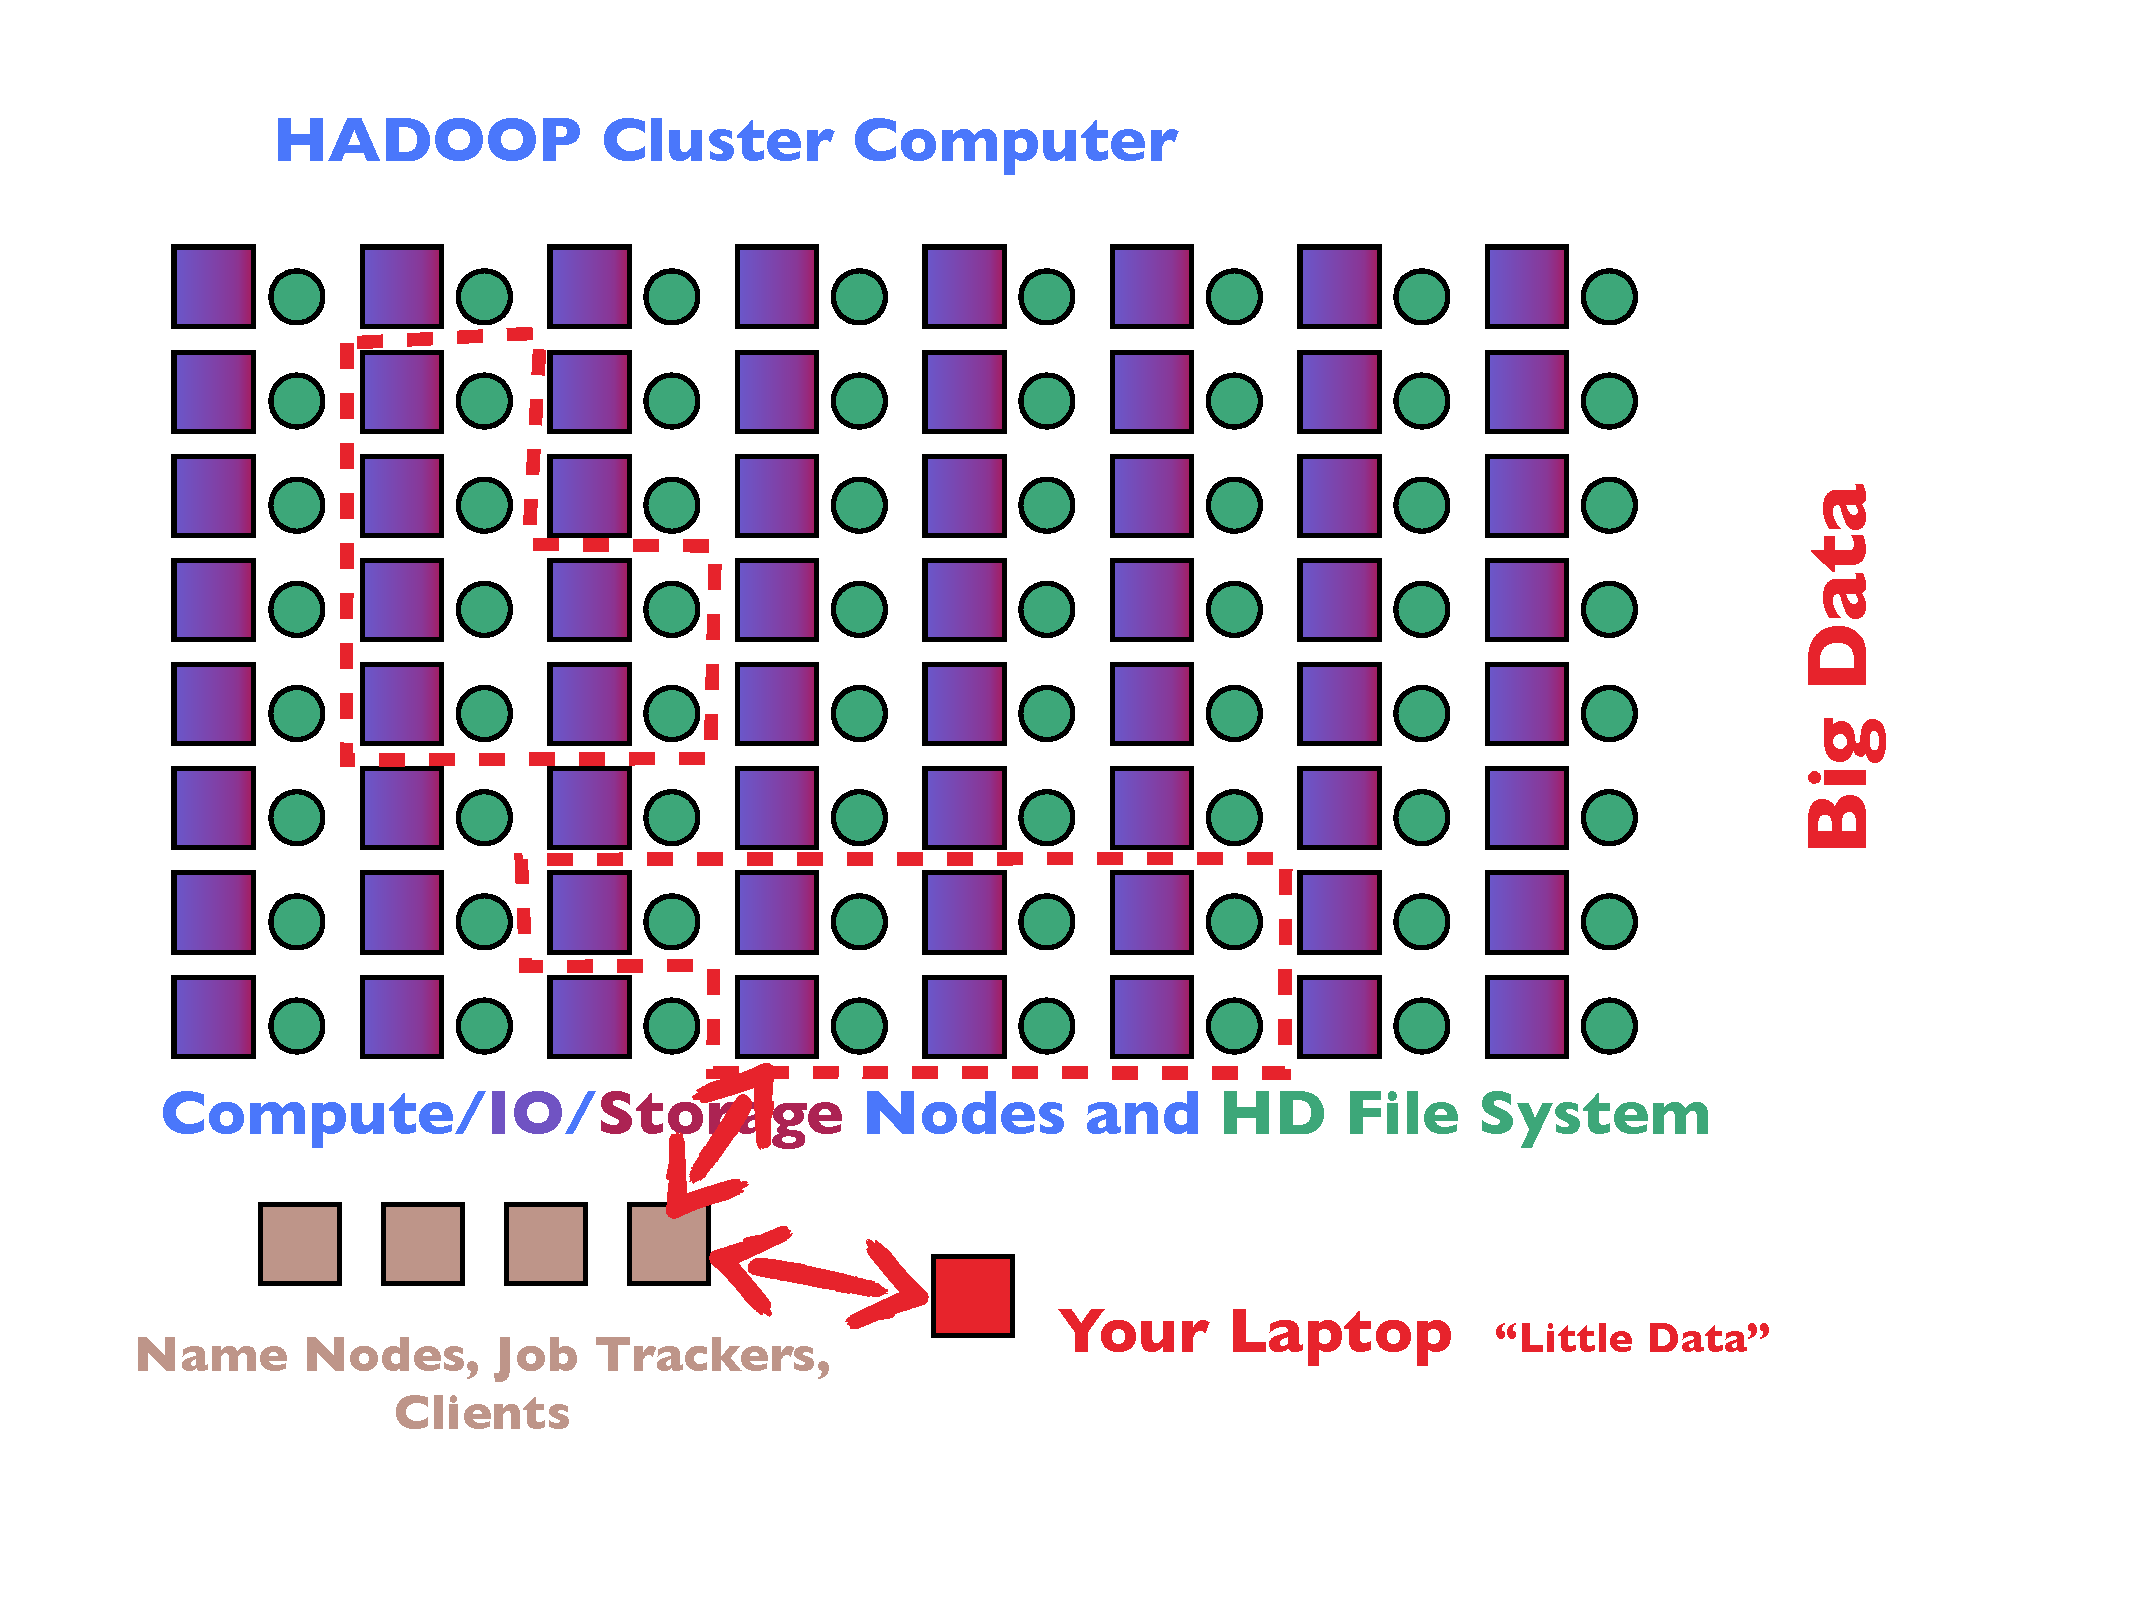
\includegraphics[trim=2cm 0cm 0cm 0cm,clip=true,height=0.8\textheight]
  {../common/pics/hardware/ParallelHardware23.pdf}
\end{minipage}
\begin{minipage}{3cm}\small
  \begin{block}{Components}\pause
%    \begin{itemize}[<+-|alert@+>]
    \scriptsize HDFS file system\\
    Yarn resource manager \\
    Map-reduce limitation
%    \end{itemize}
  \end{block}
\end{minipage}
\end{frame}

\begin{frame}{The future is here}
\includegraphics[height=0.9\textheight]
{../common/pics/hardware/ParallelHardware24.pdf}
\end{frame}

%\begin{frame}{\pbdR Interfaces to Libraries: Sustainable Path}
%\includegraphics[height=1.05\textheight]
%{../common/pics/hardware/ParallelHardware14.pdf}
%\end{frame}

%\begin{frame}{Low level R Interfaces to Native Tools}
%\includegraphics[width=0.95\textheight]
%{../common/pics/hardware/ParallelHardware22.pdf}
%\includegraphics[width=0.95\textheight]
%{../common/pics/hardware/ParallelHardware23.pdf}
%\end{frame}



\subsection{Batch and Interactive}
\makesubcontentsslidessec

\begin{frame}
  \begin{block}{Data analysis is interactive!}
    \pause
    \begin{itemize}[<+-|alert@+>]
    \item Data reduction to knowledge
    \item Iterative process with same data
      \begin{itemize}
      \item Exploration, model construction
      \item Diagnostics of fit and quantification of uncertainty
      \item Interpretation
      \end{itemize}
    \item S (and R) interactive ``answer'' to batch data analysis
    \item Efficient use of expensive people
    \end{itemize}
  \end{block}
  \begin{block}{Big platform computing is batch!}
    \pause
    \begin{itemize}[<+-|alert@+>]
    \item Libraries built for batch computing
    \item Traditionally data generation by simulation science
    \item Efficient use of expensive platforms
    \end{itemize}
  \end{block}
\end{frame}

\begin{frame}
  \begin{block}{High-Level Language: Batch and Interactive Distinction Blurred.}
    \begin{itemize}
    \item A function is a ``batch'' script
    \item \R ``An interactive environment to use batch scripts''
    \end{itemize}
  \end{block}
  \begin{block}{Ideal solution: Interactive Client with a Batch
      Server}
    \begin{itemize}
    \item Parallel visualization systems (VisIt and ParaView) are
      client-server (batch on server)
    \item Current \pbdR packages address server side (batch)
    \item pbdCS 0.1-0 released on GitHub
      \begin{itemize}
      \item Interactive SPMD
      \item Based on ZeroMQ distributed messaging (pbdZMQ 0.1-1 on CRAN)
      \item Bridge resource manager (pbdSCHED 0.1-0 on GitHub)
      \item Site configuration file
      \item Manage relationship of big data (server side) to little
        data (client side)
      \end{itemize}
    \end{itemize}
  \end{block}
\end{frame}


\subsection{Programming Models}
\makesubcontentsslidessec

\begin{frame}{Manager-Workers}
  \begin{block}{}
    \begin{itemize}
    \item A serial program (Manager) divides up work and/or data
    \item Workers run in parallel without interaction
    \item Manager collects/combines results from workers
    \item Divide-Recombine fits this model
    \end{itemize}
  \end{block}
\end{frame}

\begin{frame}{MapReduce}
  \begin{block}{}
    \begin{itemize}
    \item A concept born of a search engine
    \item Decouples certain coupled problems with an intermediate
      communication - shuffle
    \item User writes two serial codes: Map and Reduce
    \end{itemize}
  \end{block}
\end{frame}

\begin{frame}{MapReduce: a Parallel Search Engine Concept}
  \begin{block}{Search MANY documents \hfill Serve MANY users}
    \begin{center}\scriptsize
      \begin{equation*}
        \begin{array}{c@{\hspace{-2ex}}r@{\hspace{-2ex}}c}
          \begin{array}{c}
            \mbox{\scriptsize Web} \\
            \mbox{\scriptsize Pages} \\
            \mbox{\scriptsize (records)}
          \end{array} &
          \begin{array}{c}\tiny
            \\ \mbox{\tiny p0} \\ \mbox{\tiny p1} \\
            \mbox{\tiny p2} \\ \mbox{\tiny p3}
          \end{array} &
          \begin{array}{c}
            \mbox{\scriptsize Index Words (keys)} \\
            \left[
            \begin{array}{cccc}
              A_1 & A_2  & A_3 & A_4 \\
              \hline
              B_1 & B_2  & B_3 & B_4 \\
              \hline
              C_1 & C_2  & C_3 & C_4 \\
              \hline
              D_1 & D_2  & D_3 & D_4
            \end{array}
            \right]
          \end{array}
        \end{array}
        \hbox{\hspace{-2ex}}
        \begin{array}{c}
          \hbox{Shuffle} \\
          \longrightarrow \\
          \mbox{\code{MPI\_Alltoallv}}
        \end{array}
        \hbox{\hspace{-2ex}}
        \begin{array}{c@{\hspace{-2ex}}r@{\hspace{-2ex}}c}
          \begin{array}{c}
            \mbox{\scriptsize Index} \\
            \mbox{\scriptsize Words} \\
            \mbox{\scriptsize (keys)}
          \end{array} &
          \begin{array}{c}
            \\  \mbox{\tiny p0} \\ \mbox{\tiny p1} \\
            \mbox{\tiny p2} \\ \mbox{\tiny p3}
          \end{array} &
          \begin{array}{c}
            \mbox{\scriptsize Web Pages (records)} \\
            \left[
            \begin{array}{cccc}
              A_1 & B_1  & C_1 & D_1 \\
              \hline
              A_2 & B_2  & C_2 & D_2 \\
              \hline
              A_3 & B_3  & C_3 & D_3 \\
              \hline
              A_4 & B_4  & C_4 & D_4
            \end{array}
            \right]
          \end{array}
        \end{array}
      \end{equation*}
    \end{center}
    \vspace{2em}
    \begin{center}
      Matrix transpose in another language?
    \end{center}
  \end{block}
\end{frame}

\begin{frame}
  \begin{block}{Can use different sets of processors}
    \begin{center}
      \begin{equation*}\scriptsize
        \begin{array}{c@{\hspace{-2ex}}r@{\hspace{-2ex}}c}
          \begin{array}{c}
            \mbox{\scriptsize Web} \\
            \mbox{\scriptsize Pages} \\
            \mbox{\scriptsize (records)}
          \end{array} &
          \begin{array}{c}\tiny
            \\ \mbox{\tiny p0} \\ \mbox{\tiny p1} \\
            \mbox{\tiny p2} \\ \mbox{\tiny p3}
          \end{array} &
          \begin{array}{c}
            \mbox{\scriptsize Index Words (keys)} \\
            \left[
            \begin{array}{cccc}
              \\
              \hline
              B_1 & B_2  & B_3 & B_4 \\
              \hline
              \\
              \hline
              \\
            \end{array}
            \right]
          \end{array}
        \end{array}
        \hbox{\hspace{-2ex}}
        \begin{array}{c}
          \hbox{Streaming} \\
          \hbox{Shuffle} \\
          \longrightarrow \\
          \mbox{\code{MPI\_Scatter}}
        \end{array}
        \hbox{\hspace{-2ex}}
        \begin{array}{c@{\hspace{-2ex}}r@{\hspace{-2ex}}c}
          \begin{array}{c}
            \mbox{\scriptsize Index} \\
            \mbox{\scriptsize Words} \\
            \mbox{\scriptsize (keys)}
          \end{array} &
          \begin{array}{c}
            \\  \mbox{\tiny p4} \\ \mbox{\tiny p5} \\
            \mbox{\tiny p6} \\ \mbox{\tiny p7}
          \end{array} &
          \begin{array}{c}
            \mbox{\scriptsize Web Pages (records)} \\
            \left[
            \begin{array}{cccc}
              \quad  & B_1  & \quad & \quad \\
              \hline
              \quad  & B_2  & \quad  &  \quad \\
              \hline
              \quad  & B_3  & \quad  &  \quad \\
              \hline
              \quad  & B_4  & \quad  & \quad
            \end{array}
            \right]
          \end{array}
        \end{array}
      \end{equation*}
    \end{center}
  \end{block}
\end{frame}

\begin{frame}{MPI and MapReduce}
  \begin{block}{Both Concepts are about Communitation}
    \begin{itemize}
    \item One makes communication explicit, gives choices
    \item The other hides communication, gives one choice (shuffle)
    \end{itemize}
  \end{block}
\end{frame}

\begin{frame}{SPMD: Single Program Multiple Data}
  \begin{block}{}
    \begin{itemize}
    \item The prevalent way of distributed programming
    \item Can handle tightly coupled parallel computations
    \item It is designed for batch computing
    \item There is usually no manager - rather, all cooperate
    \item Prime driver behind MPI specification
    \end{itemize}
  \end{block}
\end{frame}

\begin{frame}{Early SPMD Work in Statistics: Crossproduct (Row-Block)}
  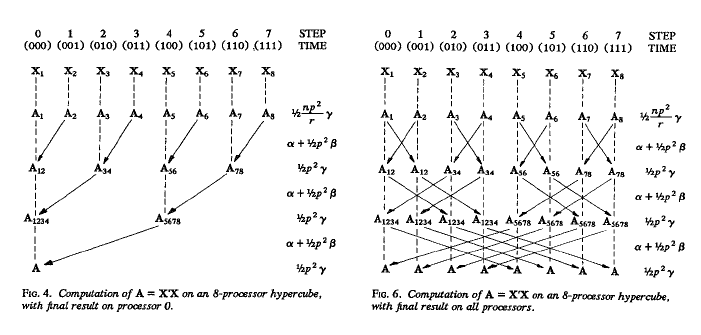
\includegraphics[width=\textwidth]
  {../common/pics/comm/Crossprod1987.png} \\
  \begin{block}{Hypercube: Individual send() and recv() over each dimension}
    {\scriptsize Ostrouchov (1987). Parallel Computing on a
      Hypercube: An overview of the architecture and some
      applications. {\em Proceedings of the 19th Symposium on the
        Interface of Computer Science and Statistics}, p.27-32.}
  \end{block}
\end{frame}

\begin{frame}{Simplified with MPI (and further with pbdMPI)}
  \includegraphics[trim=0cm 6cm 0cm 4cm,clip=true,width=\textwidth]
  {../common/pics/comm/ParallelHardware30.pdf}
  \vspace{-1ex}
  \begin{block}{Architecture-specific vendor optimizations}
    \begin{itemize}
    \item \small Cray MPT
    \item \small SGI MPT
    \end{itemize}
  \end{block}
\end{frame}

\begin{frame}{Data-flow: Parallel Runtime Scheduling and Execution
    Controller (PaRSEC)}
  \vspace{-.1cm}
  \hspace{2cm}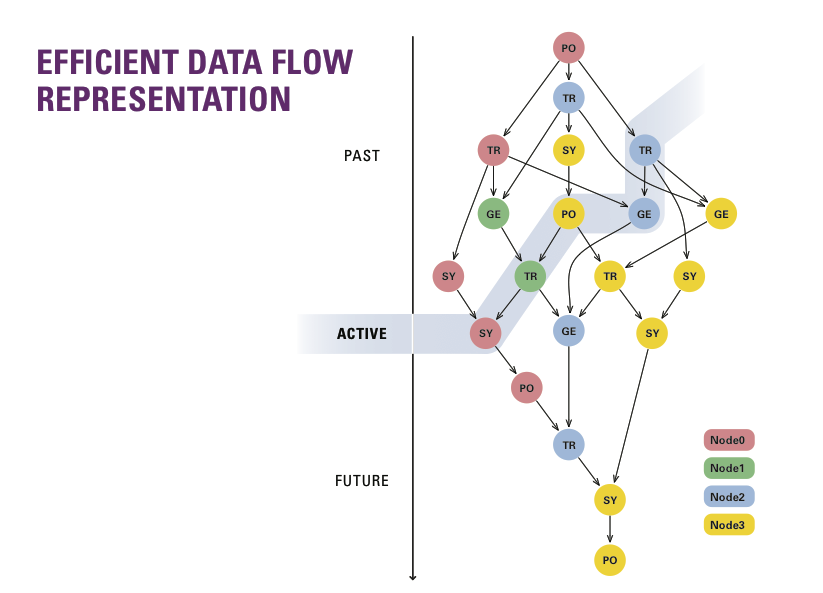
\includegraphics[trim=0cm 0cm 0cm
  1cm,clip=true,width=7.5cm]{../common/pics/comm/PaRSEC1.png}
 \\[-3.4cm]
  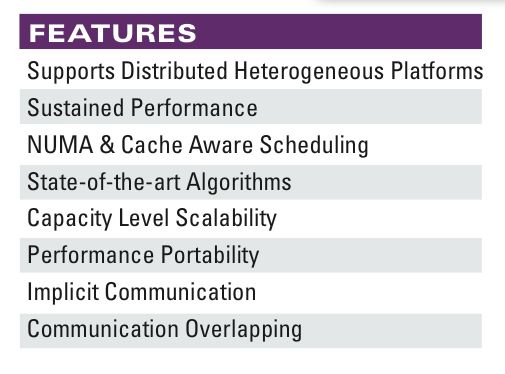
\includegraphics[width=4cm]{../common/pics/comm/PaRSEC2.png}
  \hspace{5cm}{\tiny Graphic from icl.cs.utk.edu}
  \begin{block}
    {\tiny Bosilca, G., Bouteiller, A., Danalis, A., Faverge,
      M., Herault, T., Dongarra, J. "PaRSEC: Exploiting Heterogeneity
      to Enhance Scalability," IEEE Computing in Science and
      Engineering, Vol. 15, No. 6, 36-45, November, 2013.}
    \begin{itemize}\small
    \item Master data-flow controller runs distributed on all cores.
    \item Dynamic generation of current level in flow graph
    \item Effectively removes collective synchronizations
    \end{itemize}
  \end{block}
\end{frame}

\lsc{Interacting with Nautilus}
A complete set of documentation on connecting to Nautilus can be found at the \href{http://www.nics.tennessee.edu/getting-started/access}{the access page on the NICS site}.  We will provide some examples that should illustrate the process sufficiently for users, but if there is ambiguity, you are always encouraged to check the \href{http://www.nics.tennessee.edu}{NICS site} documentation.

\lsuc{Connecting to Nautilus}
In order to connect to and use Nautilus, you must have a \textbf{S}ecure \textbf{SH}ell (SSH) client.  SSH is a protocol that allows encrypted connections between remote computers.  It consists of two parts, the ssh server (Nautilus) and the ssh client (your computer).

\subsubsection{Connecting from Mac and Linux}\label{confml}
Mac OS X and Linux have a ssh client bundled with the operating system.  On a Mac, you can open a terminal by navigating to your Applications folder, then the Utilities folder, and running the app ``Terminal''.  On Linux, the method for starting a terminal will depend to some degree on your distribution of choice.\\\\
%
If you would prefer, you can also use Putty (see section \ref{confromwin} below) as it is multiplatform (although this is not necessary).  It provides a graphical user interface for starting (but not using) a terminal session.  For the remainder, we will not assume that you are using Putty (though if you are, it should be reasonably clear how to take the information here and use it appropriately in Putty; alternatively, see section \ref{confromwin} below).\\\\
%
For demonstration purposes, say your username for your Nautilus account is \texttt{nautuser}.  Exactly how you connect will depend on whether you have an XSEDE account or a Director's Discretion account from section \ref{getacct}.  If you have an XSEDE account, then you would enter into the terminal:
\begin{lstlisting}[language=sh]
ssh nautuser@login.nautilus.nics.xsede.org
\end{lstlisting}%%%
On the other hand, if you have a Director's Discretion account, you would login by entering into the terminal:
\begin{lstlisting}[language=sh]
ssh nautuser@login.nautilus.nics.tennessee.edu
\end{lstlisting}%%%

Of course, it is inconvenient to type this into the terminal every time, so you may wish to configure a ``shortcut'' of sorts.  To do this, you would need to create a file called \texttt{config} and put that in the \texttt{.ssh/} (note the preceding dot) subdirectory of your home directory.  If this directory does not exist, create it.  With your text editor of choice, you might enter into this config file:\\\\
%
\texttt{ Host nautilus\\
HostName login.nautilus.nics.xsede.org\\
User nautuser\\
TCPKeepAlive yes\\
}

filling in the appropriate information as needed, so that to connect you need only type
\begin{lstlisting}[language=sh]
ssh nautilus
\end{lstlisting}%%%
into the terminal.\\\\
%
However you choose to go about it, begin an ssh session with Nautilus.  On your first login, you will be prompted about adding a RSA key to your cache.  Do so.


See section \ref{nautpw} below for complete details about your password.

\subsubsection{Connecting from Windows}\label{confromwin}
Windows users will have to download an ssh client, such as \href{http://www.chiark.greenend.org.uk/~sgtatham/putty/}{Putty}.  For a complete set of Putty documentation, see \href{http://the.earth.li/~sgtatham/putty/0.62/htmldoc/}{the putty user manual}.\\\\
%
After starting putty, you will need to enter the Nautilus host name under the Session category.  Make sure that the connection type is set to SSH and that the port is 22.  Which host name you use will depend on which type of account you created in section \ref{getacct}.  If you have an XSEDE account, then you would use the hostname\\\\
%
\texttt{login.nautilus.nics.xsede.org}
\\\\
On the other hand, if you have a Director's Discretion account, you would login by entering into the terminal:\\\\
%
\texttt{login.nautilus.nics.tennessee.edu}
\\\\
You can save this session either as the default or under the name of your choosing.  There are many configurable options available to you in Putty, but they are not needed to proceed (though altering them may make your experience more enjoyable).\\\\
%
Your first time connecting you will be greeted with a warning about a secure RSA key.  Select the option to add the key to Putty's cache.  You will then be greeted by a prompt asking what name you wish to login as.  Enter the account name from the account creation step and press enter.  You will then be asked to enter your password.  See section \ref{nautpw} below for complete details about your password.

\subsubsection{Your Nautilus Password}\label{nautpw}
Your password for the Nautilus system will consist of two pieces:  your PIN that you set in the account creation process, and the number that shows on your NICS token.  For illustration, say your PIN is 1234 (do not make this your PIN) and your NICS token reads 567 890.  Then the password you would enter when prompted would be 1234567890.\\\\
%
The number displayed on your NICS token will change roughly every 30 seconds (the little bars on the lower left will give you a sense for how much longer you have with that particular set of digits).  For more information, see the \href{http://www.nics.tennessee.edu/getting-started/access#OTPAuthentication}{access page on the NICS site}.


\lsuc{Basic Commands}
Once you are connected to Nautilus, you will be greeted by a text prompt.  If this is your first interaction with such a system, you may have no idea how to proceed.  This part can be confusing at first, but with a little time and patience, it will become second nature to you.\\\\
%
When interacting with the shell, never forget that it is case sensitive.  The table below
\begin{table}[h]
 \centering
  \begin{tabular}{lll}\hline
   command & description & example\\\hline
   ls & list files in a directory & ls\\
   mkdir & make directory & mkdir dir\\
   cd & change directory & cd dir\\
   cp & copy a file & cp a b\\
   mv & move and/or rename a file & mv a dir\\
   man & the help system & man mv\\\hline       
  \end{tabular}
\end{table}  
provides the basic commands you will need most of the time.\\\\
%
Never be afraid to read the man pages.  If you ever find yourself wondering ``is it possible to'', the answer is yes, and it's probably an option explained in the man page for the program.  To search within a man page, use the \texttt{/} key followed by your query.  If there are multiple hits for your query, you can jump to the next one by pressing \texttt{n} and to the previous one with \texttt{N}.

  \lsuc{Loading Software}
Much of the software available on Nautilus must first be loaded by the user before it can be used.  If you enter the command
\begin{lstlisting}[language=sh]
R
\end{lstlisting}%%%
into the terminal (remember, case sensitive), you will get the message
\begin{lstlisting}[language=sh]
-bash:  R:  command not found
\end{lstlisting}%%%
assuming your shell is bash.  At any time you can see which shell you are using by entering the command
\begin{lstlisting}[language=sh]
file /bin/sh
\end{lstlisting}%%%
So how do we start R?  You must first load R through the module system.  To do so, you would enter the command
\begin{lstlisting}[language=sh]
module load r
\end{lstlisting}%%%
into the terminal, and R will now start as expected after entering the ``R'' command into the terminal.  You only have to use the module load command once per login session (but you must load R again after a disconnect).  
\begin{lstlisting}[language=sh]
module load r
R
\end{lstlisting}%%%`
The module system is very powerful and very important to your life on this (or any other) supercomputer.  Entering the command
\begin{lstlisting}[language=sh]
man module
\end{lstlisting}%%%
will give you a complete description of the functionality and use of the module system.  For more information, see the \href{http://www.nics.tennessee.edu/computing-resources/nautilus/software}{Nautilus software page on the NICS site}.\\\\
%
The table below summarizes the use of the module system.

\begin{table}[h]
 \centering
\begin{tabular}{ll}\hline
Command & Purpose\\\hline
module avail & List available programs in the module system\\
module load $<$program$>$ & Load program\\
module unload $<$program$>$ & Unload program\\\hline
% module swap $<$first$>$ $<$second$>$ & Swap first program for second (in cases of confli
\end{tabular}
\end{table}

\lsuc{Choosing a Text Editor}
Choosing a text editor can be a very lengthy journey, somewhat akin to seeking out religious enlightenment.  No one text editor is perfect, and a discussion of the features of common text editors is well beyond the scope of this document.  Eventually, you will likely want to choose use either \href{https://www.gnu.org/software/emacs/}{Emacs} (no relation to Apple) or \href{http://www.vim.org/}{vim}.  Each of these is available on Nautilus each time you log in (you do not have to load them through the module system).  If you are not familiar with either of these editors, they can be very difficult to learn at first, but learning to use one of these well is a good idea.\\\\
%
For now, these might be a bit intimidating and act as one more hurdle in getting to the real work you want to do.  To that end, it might be a good idea to start with a more friendly text editor, such as nano.  Nano is not loaded by default each session, so you will have to enter the command
\begin{lstlisting}[language=sh]
module load nano
\end{lstlisting}%%%
to first load nano, and then call the editor by entering
\begin{lstlisting}[language=sh]
nano
\end{lstlisting}%%%
The commands for nano are visible at the bottom of the screen.  So here, Ctrl together with R reads in a file, Ctrl together with O saves, etc.  The editor is extremely minimalistic in terms of features, but is a fine place to start until you become more comfortable working in a terminal. \\\\
If you wish to have nano loaded each time you log in to Nautilus, you could start nano, enter Ctrl+R to bring up the read file dialogue.  For the file, enter
\begin{lstlisting}[language=sh]
~/.bashrc
\end{lstlisting}%%%
and somewhere inside this configuration file, add the line
\begin{lstlisting}[language=sh]
module load nano
\end{lstlisting}%%%
Press Ctrl+O to save the edit, and whenever you log in from now on, you do not first have to first load nano through the module system to be able to run nano.

\lsuc{Transferring Files}
To transfer files over to Nautilus, you have a variety of options, explained in depth at the \href{http://www.nics.tennessee.edu/computing-resources/data-transfer}{Data Transfer page at the NICS site}.  For getting started, probably the two methods of file transfer available that will be of interest are sftp for small files and GridFTP for big files.

\subsubsection{Small File Transfer}
If the files you wish to transfer are not particularly large (eg, small datasets, some R scripts, etc.), probably the easiest way to proceed is to connect to Nautilus by sftp (the secure file transfer protocol).  \\\\
%
Mac and Linux users can use the terminal as with ssh, and Windows users can use Putty (via PSFTP) to connect via sftp.  Although there is gui program available for managing files over sftp called \href{http://filezilla-project.org/}{filezilla}.  If you elect to use filezilla, you should read its documentation, although the program should be fairly self-explanatory.\\\\
%
To connect from a terminal (Mac/Linux), you can enter the command \texttt{sftp} as you would use \texttt{ssh} in Section \ref{confml}.  So for example, you might enter the command
\begin{lstlisting}[language=sh]
sftp nautuser@login.nautilus.nics.xsede.org
\end{lstlisting}%%%
or if you set up your ssh config file as in the example, you could do
\begin{lstlisting}[language=sh]
sftp nautilus
\end{lstlisting}%%%
From here, you can transfer files via the self-explanatory commands \texttt{put} and \texttt{get}.  The above applies for Windows users, after you replace ``sftp'' with ``psftp''.\\\\
%
Your sftp password is the same as your ssh password. 

\subsubsection{Large File Transfer}
If you need to transfer large files, such as your full dataset, using sftp is not recommended.  In this case, the preferred method is GridFTP.  You will need a special GridFTP client such as \href{https://www.globusonline.org/}{globus-url-copyh} or \href{http://dims.ncsa.illinois.edu/set/uberftp/}{uberftp}.  For details about how to set up and use GridFTP with these clients, see the \href{http://www.nics.tennessee.edu/user-support/general-support/data-transfer/gridftp}{GridFTP page on the NICS site}.


\lsc{The Job Queue System}\label{jqssec}
Generally, you will do very little direct interaction with Nautilus.  You should not really be using Nautilus in the same way that you use a workstation; it is not a workstation.  Nautilus is a shared system.  No one person is the sole user of Nautilus at any given time (usually).  \\\\
%
The way you will want to run your analyses is by submitting your job to a queue system on Nautilus.  This system handles all of the user requests and keeps the various demands for resources (cores, ram) from different jobs from stepping on each others toes, so to speak.\\\\
%
A very thorough explanation of the various options and ways of interacting with the job queue system is provided at the \href{http://www.nics.tennessee.edu/computing-resources/nautilus/Batch_Scripts}{batch scripts page on the NICS site}, and so we will not reproduce that information here.  We merely provide a quick sketch of the general process.  For full details and explanations, see the NICS site.  However, you can find some example scripts in the Examples section, Section \ref{egsec}.\\\\
%
However, there are a few options which you should be made aware of.  First, processor allocations are given by node, not by core.  On Nautilus, there are 8 cores per node, so when requesting processors for your job, you should generally request multiples of 8 (because that is what you are going to get anyway).  If you request 1 core, you will get 8; requesting 9 gets you 16, etc.  Likewise, since allocations are by node, ram is allocated similarly.  Each node has 4gb of ram per cpu, and so if you request 8 cores, you will get 32gb of ram.\\\\
%
As for dealing with the queue system, the first step is usually to create an appropriate batch file for your particular job.  This batch file will contain the information Nautilus needs to run your job.  The kind of information you will need will depend on what kind of job you wish to submit.  See the examples in section \ref{egsec} as well as the \href{http://www.nics.tennessee.edu/computing-resources/nautilus/Batch_Scripts}{batch scripts page on the NICS site}.\\\\
%
Once you have your job file prepared, you can submit it to the queue using the \texttt{qsub} command.  So if you have a job file called \texttt{jobfile.pbs} prepared and you are in the directory of this file, then you can submit it to the queue system via the command
\begin{lstlisting}[language=sh]
qsub jobfile.pbs 
\end{lstlisting}%%%
You can check on your job via the commands \texttt{showq} and \texttt{qstat}, but will probably want to use the job file options to send out emails to you.\\\\
%
Finally, if you ever need to prematurely kill a job (whether it is running or merely queued), you can do so with the \texttt{qdel} command.
\lsc{R on Nautilus}
Performing an analysis with R on a remote system can be challenging at first.  The aim of this section is to help with the transition of specifically running R for analysis on a local desktop system to running R on a remote parallel system.

\lsuc{Packages and Libraries}

\subsubsection{Using the Existing Library}
Installing packages, especially complicated ones like Rmpi and gputools, can be difficult on a remote system, especially for the R user who may have never had to deal with compiling things before.  Thankfully, many of the packages you will want to use are already installed for you.  If we are using R version 2.12.0, then the default library path is
\begin{lstlisting}[language=sh]
/sw/analysis/r/2.12.0/sles11.1\_intel11.1/R-2.12.0/library} 
\end{lstlisting}%%%
So merely loading R via the module system and then, for instance, if you want to use the \texttt{multicore} library, since this is already in the default library, all you have to do is
\begin{lstlisting}[language=rr]
library(multicore)
\end{lstlisting}
If you require an additional package which is not currently installed, the simplest way to get this is to fill out a request at the \href{http://www.nics.tennessee.edu/software-request}{Request Software Installation page at the NICS site}.

\subsubsection{Managing Your Own R Library}
You can also of course manage your own R library, though for most this will at best be unnecessary, and at worst a needless, frustrating exercise.  If you do need to manage, at least in part, your own R library, then you must install packages from source, either by downloading the source package (say with the utility wget) and install it with the command
\begin{lstlisting}[language=sh]
R CMD INSTALL [options] packages
\end{lstlisting}%%%
or by using the \texttt{install.packages()} command in an interactive R session, setting the various options as needed (\texttt{lib=}, \texttt{INSTALL\_opts=}, \dots).  One option that is not optional (without overriding an R environment variable; see paragraph to follow for details) when installing a package to a custom, user-managed library is the \texttt{lib=} argument.  This is so because you do not have write access to your default library.  Similarly, to load a package from a custom library, make sure you set the appropriate \texttt{lib.loc=} argument when issuing the \texttt{library()} command in R.\\\\
%
One additional note to consider when maintaining your own R package library is that you will likely need to manually set a few R environment variables in order to get some packages to install, or even load.  For a mostly complete list of R environment variables, enter the command \texttt{help("environment variables")} in an interactive R session.

\lsuc{Different R Versions}
For more information, see the \href{http://www.nics.tennessee.edu/computing-resources/nautilus/software?&software=r}{R page at the NICS site}.

\lsuc{Running Batch Jobs}
As mentioned in Section \ref{jqssec}, you generally should not be running R in quite the same way that you would run it on your workstation.  On your workstation, you probably use R interactively; that is, you load up an R session and submit lines to the R terminal as you need. \\\\
%
By contrast, on Nautilus, you will be running R scripts in batch.  That is, you will not start an interactive R session.  Instead, you will issue a command from the terminal (really, from you job script) to start R, run your analysis, direct output to a file, and kill R when the script completes (or encounters an error).  Now, for the purposes of appropriate resource allocation, this should be be done in your jobfile that you submit via qsub, rather than directly handled in the terminal.  This is merely intended to illustrate what is actually going on.  \\\\
%
One way to do this is to issue the terminal command \texttt{R CMD BATCH}.  So say the script you wish to have R run is called \texttt{myscript.R}.  Then issuing the command
\begin{lstlisting}[language=sh]
R CMD BATCH myscript.R 
\end{lstlisting}%%%
will run the \texttt{myscript.R} script through R in a way that is somewhat equivalent to starting an interactive R session and issuing the R commands 
\begin{lstlisting}[language=rr]
sink("myscript.Rout")
source("myscript.R")
q(save="no")
\end{lstlisting}

% \lsuc{Starting an interactive R session}
% Most of the time when you use R on Nautilus, you should submit a batch job via the queue system.  However, on occasion you may need to run R interactively (like you would on your own computer).  

% \input{05{parallelr}
% 
\lsc{Examples}\label{egsec}
  \lsuc{A Monte Carlo Simulation}
You are probably familiar with the Monty Hall problem from the game show Let's Make a Deal.  If not, you might wish to read the \href{https://en.wikipedia.org/wiki/Monty_Hall_problem}{Wikipedia page} devopted to this problem.  A brief explanation is that the contestant is shown three doors to choose between.  Behind only one door is a prize.  The contestant chooses a door, and from the unchosen 2 doors, one is removed from play.  The contestant is then asked if he or she would like to switch from the initially chosen door to the only remaining door.  What is the probability of winning if the contestant switches?\\\\
%
We can easily simulate a play of this game with the R function \texttt{f()} defined as
\begin{lstlisting}[language=rr]
# Single game, assuming the player always switches
f <- function(.){
  prize.door <- sample(1:3, size=1)
  choice <- sample(1:3, size=1)

  if (choice==prize.door) return(0) else return(1) # Always switch
}
\end{lstlisting}

This is not necessarily the most efficient way to proceed.  Generally calling functions is costly, so it might make more sense to develop \texttt{f()} to take a ``number of runs'' argument, and this would probably improve the performance somewhat.  However, proceeding in our fashion is, for the sake of example, somewhat easier to follow in the various parallel implementations.

\subsubsection{Serial}
With the function \texttt{f} as above, it we can use \texttt{lapply()} to evaluate many runs
\begin{lstlisting}[language=rr]
n <- 1e7 # number of trials

system.time({
  mean(unlist(lapply(X=1:n, FUN=f)))
})
\end{lstlisting}
If this code is stored in the file serial.R, then you might submit it to Nautilus via the job file (remember to change ``your-account-number'' below to your actual account number.  Use the command \texttt{showusage}):
\begin{lstlisting}[language=sh]
#PBS -N Serial_sim_example
#PBS -S /bin/bash
#PBS -A your-account-number
#PBS -j oe
#PBS -l ncpus=8
#PBS -l walltime=1:00:00
#PBS -q analysis

module load r

R CMD BATCH serial.R
\end{lstlisting}%%%
Notice that we are asking for 8 cores, even though we are only going to use 1.  Remember that asking for 1 really takes 8 anyway.\\\\
%
Submitting this job results in the run time:
\begin{lstlisting}[language=rr]
   user  system elapsed 
187.275   0.220 187.516 
\end{lstlisting}


\subsubsection{Multicore}
With multicore, there is not much that we have to change over the serial implementation
\begin{lstlisting}[language=rr]
n <- 1e7 # number of trials
cores <- 10 # number of cores

library(multicore)

system.time({
  # mclapply() instead of lapply()
  mean(unlist(mclapply(X=1:n, FUN=f, mc.cores=cores)))
})
\end{lstlisting}

The \texttt{mclapply()} functions has the option \texttt{set.seed=} which defaults to \texttt{TRUE}.  This ensures that parallel processes have different seeds, which of course is very important for Monte Carlo simulation, since otherwise independence of the trials is violated.\\\\
%
If this code is stored in the file multicore.R, then you might submit it to Nautilus via the job file:

\begin{lstlisting}[language=sh]
#PBS -N Multicore_sim_example
#PBS -S /bin/bash
#PBS -A your-account-number
#PBS -j oe
#PBS -l ncpus=8
#PBS -l walltime=1:00:00
#PBS -q analysis

module load r
export TMPDIR=$HOME
export LC_ALL=C

cd $PBS_O_WORKDIR
R CMD BATCH multicore.R
\end{lstlisting}%%%
Submitting this job results in the run time:
\begin{lstlisting}[language=rr]
   user  system elapsed 
162.329   2.208  61.459 
\end{lstlisting}


\subsubsection{SNOW}
\begin{lstlisting}[language=rr]
n <- 1e7 # number of trials
cores <- 10 # number of cores

library(rlecuyer) # for parallel rng
library(snow)

system.time({
  # set up the workers
  cl <- makeCluster(cores, type="SOCK")
  
  # Pass objects to the workers
  clusterExport(cl, c("n", "cores", "f"))

  # parLapply() instead of lapply()
  mean(unlist(parLapply(cl=cl, x=1:n, fun=f)))
  stopCluster(cl)
})
\end{lstlisting}

If this code is stored in the file snow.R, then you might submit it to Nautilus via the job file:

\begin{lstlisting}[language=sh]
#PBS -N SNOW_sim_example
#PBS -S /bin/bash
#PBS -A your-account-number
#PBS -j oe
#PBS -l ncpus=8
#PBS -l walltime=1:00:00
#PBS -q analysis

module load r

R CMD BATCH snow.R
\end{lstlisting}%%%
Submitting this job results in the run time:
\begin{lstlisting}[language=rr]
   user  system elapsed 
 86.069   2.720 124.031 
\end{lstlisting}


\subsubsection{Rmpi}
Generally speaking, Rmpi is a bit trickier.  MPI is very powerful, and with that power comes a slightly more complicated API than with those above.  Since Nautilus is a shared memory machine, there is no real advantage to using Rmpi over Multicore; generally you should expect the runtimes to roughly be the same.  However, if you are on a distributed memory cluster, then there is only so much you can do with Multicore.  \\\\
%
Multicore operates on one node, with as many cores used within that node as possible/requested.  Nautilus is basically one big node, so Multicore can utilize all of its cores.  On a distributed memory cluster, this is not so, and the number of cores that can be utilized by Multicore will be significantly lower than can be utilized by Rmpi, and whence the potential speedup gained by Multicore on such systems pales in comparison for very big jobs.\\\\
%
Here there is a very important difference over Multicore and SNOW.  We \emph{must} make explicit steps to ensure that the random number generation operates appropriately on the workers.  Here, we do so with the \href{http://cran.r-project.org/web/packages/rlecuyer/index.html}{rlecuyer} package for R.  This can also be done with the \href{http://cran.r-project.org/web/packages/rsprng/index.html}{rsprng} package.\\\\
%
Here for consistency with the previous examples, we will use \texttt{mpi.parLapply()}, though arguably \texttt{mpi.parSim()} is more appropriate.  \\\\
%
See the \href{http://cran.r-project.org/web/packages/Rmpi/Rmpi.pdf}{rmpi documentation} for more details about the Rmpi API.
\begin{lstlisting}[language=rr]
n <- 1e7 # number of trials

library(rlecuyer) # for parallel rng
library(Rmpi)

system.time({
  mpi.spawn.Rslaves(needlog = FALSE)

  # set up parallel rng on the slaves
  mpi.setup.rngstream() 

  # mpi.parLapply() instead of lapply()
  mean(unlist(vec <- mpi.parLapply(x=1:n, fun=f)))
})

mpi.close.Rslaves(dellog = FALSE)
mpi.exit()
\end{lstlisting}

If this code is stored in the file rmpi.R, then you might submit it to Nautilus via the job file:

\begin{lstlisting}[language=sh]
#PBS -N Rmpi_sim_example
#PBS -S /bin/bash
#PBS -A your-account-number
#PBS -j oe
#PBS -l ncpus=8
#PBS -l walltime=1:00:00
#PBS -q analysis

module load r
module swap mpt mpt/2.04
export LC_ALL=C
export TMPDIR=$PBS_O_WORKDIR

cd $PBS_O_WORKDIR
mpirun -np 8 Rscript rmpi.R
\end{lstlisting}%%%
Submitting this job results in the run time:
\begin{lstlisting}[language=rr]
   user  system elapsed 
 99.370   1.088 100.581 
\end{lstlisting}


\lsuc{Linear Model Selection}
For the remainder, example job scripts will be suppressed, since they are effectively the same as those found in the examples above.\\\\
%
In this example, we will randomly generate a random normal response variable $y$, 10 random normal predictor variables $x$ and evaluate all possible $2^{10} -1 = 1023$ models which contain at least one predictor variable and choose a best model by the \href{https://en.wikipedia.org/wiki/Bayesian_information_criterion}{Bayesian Information Criterion}.\\\\
%
First we need to generate the data.  Since this is not the focus of this demonstration, we will do it once, independent of the parallel implementation.  
\begin{lstlisting}[language=rr]
n <- 1e7 # number of rows to generate

# The data
nvars <- 10
x <- matrix(rnorm(n*nvars), ncol=nvars)
y <- rnorm(n)

write.csv(data.frame(x, y), "simdata.csv")
\end{lstlisting}
A quick word of warning, it is possible that some of the models will have infinite likelihood, and no extra precaution is taken in the code to follow to prevent such an occurrence.  If you are getting strange errors, try generating a new dataset.  \\\\
%
Once this dataset has been generated, we can use the same simulated data each time in our testing of various parallel implementations.

\subsubsection{Serial}
Here, we will just have a single \texttt{for} loop that will run through the models one at a time.  This is not necessarily efficient, even ignoring running things in parallel, but this is the simplest way one might prototype a solution to this problem.  \\\\
%
For each model to be evaluated, the model is fit and its BIC score is calculated.  A comparison is made to that BIC score and the yet lowest observed BIC, and if the model BIC is lower than the previous best BIC, then we make that model the new best.

\begin{lstlisting}[language=rr]
# Read in the data
df <- read.csv("simdata.csv")
x <- as.matrix(df[1:10])
y <- as.matrix(df[11])

# Generate the list of models to evaluate
col.opt <- lapply(X=1:ncol(x), FUN=function(.) 0:1)
models.list <- expand.grid(col.opt)
models.list <- models.list[-1, ] # prune first row

# Fit the models
system.time({
  best <- Inf
  for (i in 1:nrow(models.list)){
    subst <- which(models.list[i, ] == 1)
    test <- BIC(lm(y~x[, subst]))
    if (test < best) {
      best <- test
      best.subst <- subst
    }
  }
})

# Print the output
cat(sprintf("The optimal model is that with predictors:  %s\n", paste(paste("x", best.subst, sep=""), collapse=", ")))
cat(sprintf("With BIC:  %f\n", best))
\end{lstlisting}


\subsubsection{Multicore}\label{mcmodelsel}
Here a slight change in philosophy is required.  Instead of fitting one model at a time, we fit models independently in parallel on different cores, and each time a model is evaluated, we store in a list which model we were looking at and its corresponding BIC score.  Then after we have all of the BIC scores calculated and corresponding model information, we look through the list of all BIC scores and choose the smallest such.  The model corresponding to this BIC score is then determined from the stored subset information, and is declared to be the best model.
\begin{lstlisting}[language=rr]
# Number of cores to use
cores <- 8

# Read in the data
df <- read.csv("simdata.csv")
x <- as.matrix(df[1:10])
y <- as.matrix(df[11])

# Generate the list of models to evaluate
col.opt <- lapply(X=1:ncol(x), FUN=function(.) 0:1)
models.list <- expand.grid(col.opt)
models.list <- models.list[-1, ] # prune first row


library(multicore)

f <- function(i){
  subst <- which(models.list[i, ] == 1)
  bic <- BIC(lm(y~x[, subst]))
  return(list(bic=bic, subst=subst))
}

# Fit all models, find the best among them later
system.time({
  models <- mclapply(X=1:nrow(models.list), FUN=f)
  bics <- sapply(models, "[[", 1)

  best <- min(bics)
  best.subst <-  which(models.list[which(bics==best), ] == 1)
})

# Printing output
cat(sprintf("The optimal model is that with predictors:  %s\n", paste(paste("x", best.subst, sep=""), collapse=", ")))
cat(sprintf("With BIC:  %f\n", best))
\end{lstlisting}


\subsubsection{SNOW}
Here we use the same philosophy in the Multicore solution from \ref{mcmodelsel}, with only slight modifications for use with SNOW.
\begin{lstlisting}[language=rr]
# Number of cores to use
cores <- 8

# Read in the data
df <- read.csv("simdata.csv")
x <- as.matrix(df[1:10])
y <- as.matrix(df[11])

# Generate the list of models to evaluate
col.opt <- lapply(X=1:ncol(x), FUN=function(.) 0:1)
models.list <- expand.grid(col.opt)
models.list <- models.list[-1, ] # prune first row


library(snow)

f <- function(i){
  subst <- which(models.list[i, ] == 1)
  bic <- BIC(lm(y~x[, subst]))
  return(list(bic=bic, subst=subst))
}

# Fit all models, find the best among them later
system.time({
  # Create cluster
  cl <- makeCluster(cores, type="SOCK")

  # Pass objects to the workers
  clusterExport(cl, c("cores", "x", "y", "f", "models.list"))  
  
  models <- parLapply(cl=cl, x=1:nrow(models.list), fun=f)
  bics <- sapply(models, "[[", 1)

  best <- min(bics)
  best.subst <-  which(models.list[which(bics==best), ] == 1)

  stopCluster(cl)
})

# Printing output
cat(sprintf("The optimal model is that with predictors:  %s\n", paste(paste("x", best.subst, sep=""), collapse=", ")))
cat(sprintf("With BIC:  %f\n", best))
\end{lstlisting}

\subsubsection{Rmpi}
Using Rmpi here feels very much like using SNOW.
\begin{lstlisting}[language=rr]
# Number of cores to use
cores <- 8

# Read in the data
df <- read.csv("simdata.csv")
x <- as.matrix(df[1:10])
y <- as.matrix(df[11])

# Generate the list of models to evaluate
col.opt <- lapply(X=1:ncol(x), FUN=function(.) 0:1)
models.list <- expand.grid(col.opt)
models.list <- models.list[-1, ] # prune first row


library(Rmpi)

f <- function(i){
  subst <- which(models.list[i, ] == 1)
  bic <- BIC(lm(y~x[, subst]))
  return(list(bic=bic, subst=subst))
}

# Fit all models, find the best among them later
system.time({
  mpi.spawn.Rslaves(needlog=FALSE)

  # Pass objects to the workers
  mpi.bcast.Robj2slave(x)
  mpi.bcast.Robj2slave(y)
  mpi.bcast.Robj2slave(f)

  susbests <- mpi.parLapply(X=1:nrow(models.list), FUN=function(i) which(models.list[i, ] == 1))
  mpi.bcast.Robj2slave(subsets)
  
  models <- mpi.parLapply(x=subsets, fun=f)
  bics <- sapply(models, "[[", 1)
  
  best <- min(bics)
  best.subset <- which(models.list[which(bics==best), ] == 1)
})

mpi.close.Rslaves(dellog=FALSE)
mpi.exit()

# Printing output
cat(sprintf("The optimal model is that with predictors:  %s\n", paste(paste("x", best.subst, sep=""), collapse=", ")))
cat(sprintf("With BIC:  %f\n", best))
\end{lstlisting}

\subsubsection{foreach}
Finally, we do the same with foreach.
\begin{lstlisting}[language=rr]
# Number of cores to use
cores <- 8

# Read in the data
df <- read.csv("simdata.csv")
x <- as.matrix(df[1:10])
y <- as.matrix(df[11])

# Generate the list of models to evaluate
col.opt <- lapply(X=1:ncol(x), FUN=function(.) 0:1)
models.list <- expand.grid(col.opt)
models.list <- models.list[-1, ] # prune first row


library(foreach)
library(multicore)
library(doMC)

registerDoMC(cores=cores)

# Fit all models, find the best among them later
system.time({
  models <- foreach (i=1:nrow(models.list)) %dopar% {
    subst <- which(models.list[i, ] == 1)
    test <- BIC(lm(y~x[, subst]))

    list(test, subst)
  }

  bics <- sapply(models, "[[", 1)
  best <- min(bics)
  best.subst <-  which(models.list[which(bics==best), ] == 1)
})

# Printing output
cat(sprintf("The optimal model is that with predictors:  %s\n", paste(paste("x", best.subst, sep=""), collapse=", ")))
cat(sprintf("With BIC:  %f\n", best))
\end{lstlisting}



\end{document}
